%=========================================================================%
%    5th ...
%
%    Format: LaTeX2e.
%=========================================================================%
\documentclass{ISPIV2023_Template_Paper_Class}

%
\begin{document}
%
%
\title{Paper Title}
\author{K. T. Christensen$^{1*}$, R. J. Adrian$^2$, G. Blois$^1$}
\affiliation{
		$^1$ University/Company, Institute/Department/Division, City, Country\\
 		\vspace{7pt}
	     	$^2$ University/Company, Institute/Department/Division, City, Country\\
		\vspace{7pt}
		$^*$ corresponding.author@example.com
		}
%
\maketitle

%%%%%%%%%%%%%%%%%%%%%%%%%%%%%%%%%%%%%%%%%%%%%%%%%%
%%%%%%%%%%%%%%%%%%%%%%%%%%%%%%%%%%%%%%%%%%%%%%%%%%
\begin{abstract}
{Please use this template to create either your two-page abstract (abstract deadline: January 15, 2023) or your final full-length paper (final paper deadline: May 15, 2023). In the case of a final full paper, it should be 6--10 pages in length. Please do not include page numbers, since these will be assigned later in the conference proceedings document. Please submit the PDF file following the submission instructions to be posted  \href{https://piv.sdsu.edu/abstract-paper/}{\textbf{here}}. The pdf file should have a unique name, e.g. 'paperISPIV2023\_[name of first author]\_[submission date (e.g.: Jan012023)].pdf'. Again, either a two-page abstract or a final full-length paper (if the abstract is accepted) must be submitted by their corresponding deadlines.}
\end{abstract}
%%%%%%%%%%%%%%%%%%%%%%%%%%%%%%%%%%%%%%%%%%%%%%%%%%
\section{Introduction}
\begin{figure}[h]
        \centering
    	 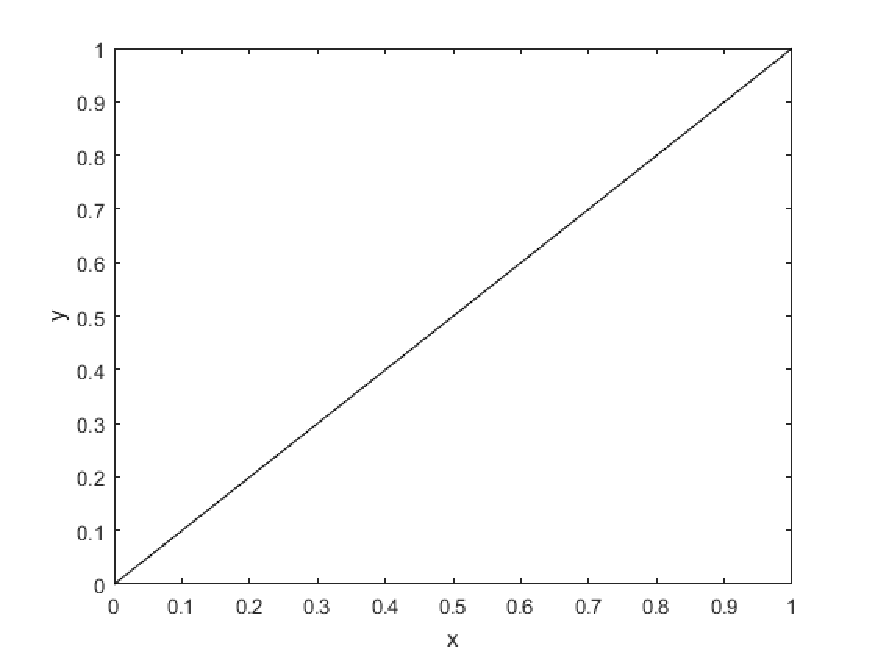
\includegraphics[width=.48\textwidth]{./figs/test.pdf}
	 \caption{This is a test figure}
        \label{fig:1}
\end{figure}
Here are three examples of citations for a book, conference proceeding and journal article: \cite{adrian2011particle}, \cite{Discetti2015}, and \cite{christensen2004influence}. Please use the provided bibliography style which is loaded in the provided document class file. 

Here is an example for an equation: the function value is calculated as
\begin{equation}
	y=m\cdot x+t
	\end{equation}
	
Figure\,\ref{fig:1} is an example for a figure. An example for a subfigure is shown in Fig.\,\ref{fig:2a}.
\begin{figure}[t]
        \centering
        \begin{subfigure}[test figure\label{fig:2a}]{
        		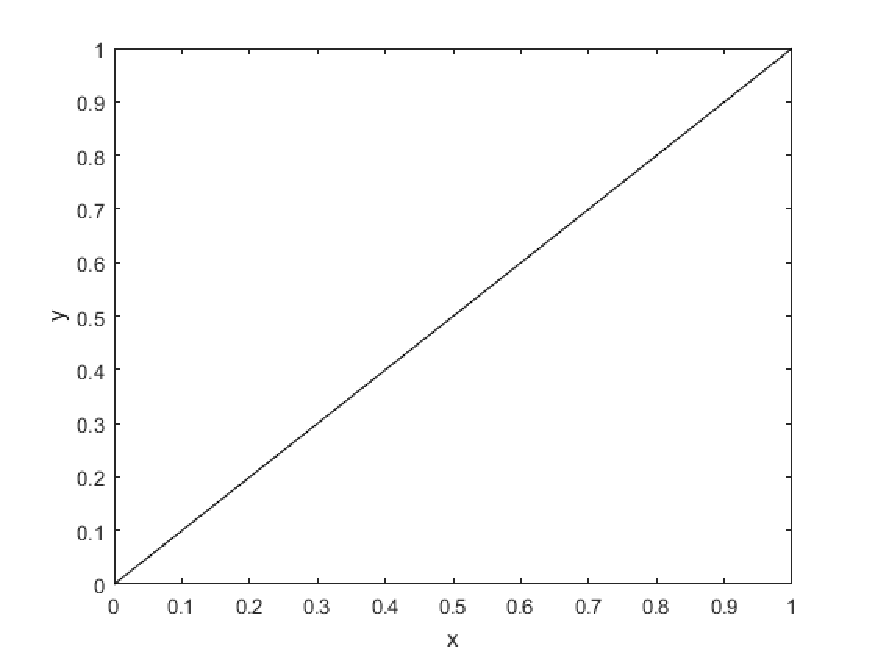
\includegraphics[width=.48\textwidth]{./figs/test.pdf}
	}
	\end{subfigure}
	\begin{subfigure}[test figure\label{fig:2b}]{
		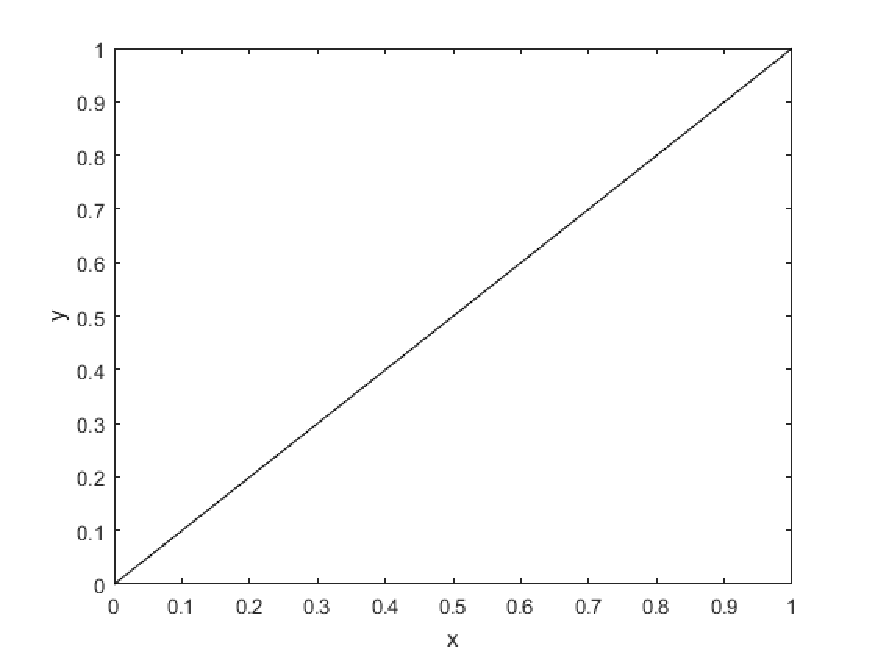
\includegraphics[width=.48\textwidth]{./figs/test.pdf}
	}
	\end{subfigure}
	\caption{Two test figures. Please try to match the font sizes in the figures with the text.}
\end{figure}
%%%%%%%%%%%%%%%% 
\section{Main Part 1}
Main Part 1. Main Part 1. Main Part 1. Main Part 1. Main Part 1. Main Part 1. Main Part 1. Main Part 1. Main Part 1. Main Part 1. Main Part 1. Main Part 1. Main Part 1. Main Part 1. Main Part 1. Main Part 1. Main Part 1. Main Part 1. Main Part 1. Main Part 1. Main Part 1. Main Part 1. Main Part 1. Main Part 1. Main Part 1. Main Part 1. Main Part 1. Main Part 1. Main Part 1. Main Part 1. Main Part 1. Main Part 1. Main Part 1. Main Part 1. Main Part 1. Main Part 1.
%%%%%%%%%%%%%%%% 
\section{Main Part X}
Main Part X. Main Part X. Main Part X. Main Part X. Main Part X. Main Part X. Main Part X. Main Part X. Main Part X. Main Part X. Main Part X. Main Part X. Main Part X. Main Part X. Main Part X. Main Part X. Main Part X. Main Part X. Main Part X. Main Part X. Main Part X. Main Part X. Main Part X. Main Part X. Main Part X. Main Part X. Main Part X. Main Part X. Main Part X. Main Part X. Main Part X. Main Part X. Main Part X.
%%%%%%%%%%%%%%%% 
\section{Conclusions}
Conclusion. Conclusion. Conclusion. Conclusion. Conclusion. Conclusion. Conclusion. Conclusion. Conclusion. Conclusion. Conclusion. Conclusion. Conclusion. Conclusion. Conclusion. Conclusion. Conclusion. Conclusion. Conclusion. Conclusion. Conclusion. Conclusion. Conclusion. Conclusion. Conclusion. Conclusion. Conclusion. Conclusion. Conclusion. Conclusion. Conclusion. Conclusion. Conclusion. Conclusion. Conclusion. Conclusion. Conclusion. Conclusion.
%%%%%%%%%%%%%%%% 
\begin{acknowledgments}
Put acknowledgments here.
\end{acknowledgments}
%%%%%%%%%%%%%%%% 
% put bibliography here
\bibliography{ISPIV2023_References}

\end{document}